
\documentclass[paper=a4, fontsize=11pt,twoside]{scrartcl}

\usepackage[a4paper,pdftex]{geometry}										% A4paper margins
\setlength{\oddsidemargin}{5mm}											% Remove 'twosided' indentation
\setlength{\evensidemargin}{5mm}

\usepackage[english]{babel}
\usepackage[protrusion=true,expansion=true]{microtype}	
\usepackage{amsmath,amsfonts,amsthm,amssymb}
\usepackage{graphicx}

\usepackage{fancyhdr}
\usepackage{hypernat}
\usepackage{hyperref}
\usepackage[small,nooneline,bf,hang]{caption} 
\parindent0cm                                  
\pagestyle{fancy}
\setcounter{tocdepth}{2}
\setcounter{secnumdepth}{3}

% macros
\newcommand{\ptat}{{pTatin3d}}
\newcommand{\shellcmd}[1]{\\\indent\indent\texttt{\hspace{5mm}\footnotesize #1}\\}
\newcommand{\unix}[1]{\texttt{\footnotesize #1}}

% Definitions for title page
\newcommand{\HRule}[1]{\rule{\linewidth}{#1}} 	% Horizontal rule

\makeatletter							% Title
\def\printtitle{%						
    {
    	\centering \@title\par}
		 	\vspace{10mm}
	\begin{figure} [hbtp]
	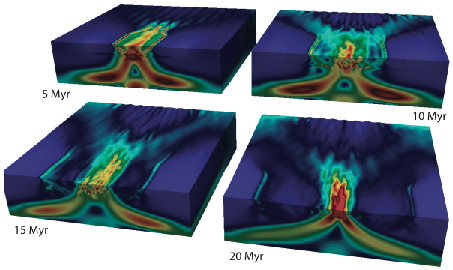
\includegraphics[height=0.4\textheight]{figs/ptat3d_front_page_small.pdf}
	\end{figure}
    }


\makeatother									

\makeatletter							% Author
\def\printauthor{%					
    {\centering \large \@author}}				
\makeatother							

%Titlepage
	\title{	\normalsize \textsc{pTatin3d Manual} 	% Subtitle of the document
	\\[2.0cm]									% 2cm spacing
	\HRule{2pt} \\ [0.3cm]						% Upper rule
	\LARGE \textbf{{pTatin3d User Guide}}			% Title
	\HRule{2pt} \\ [0.5cm]						% Lower rule + 0.5cm spacing
	\normalsize \today							% Todays date
	}

\author{
{\normalsize \textsc{Developers}}
\begin{itemize}
\item[-] Dave A. May: Institute of Geophysics, ETH Z{\"u}ruch \texttt{(dave.may@erdw.ethz.ch)} 
\item[-] Laetitia Le Pourhiet: UPMC, Univ. Paris 06  \texttt{(laetitia.le\_pourhiet@upmc.fr)}
\end{itemize}
}



\begin{document}

\thispagestyle{empty}% Remove page numbering on this page

\printtitle% Print the title data as defined above
  	\vfill
\printauthor% Print the author data as defined above


% Begin document


\newpage
\pagenumbering{roman}
\tableofcontents{}

\newpage

\pagenumbering{arabic}

\section{Overview}
{\ptat} provides a suite of functionality to study long-term geodynamic processes related to the dynamics of lithosphere and crust.
At its core, support is provided for solving non-linear, incompressible Stokes flow problems in three-dimensions using a mixed finite element method together with a marker-and-cell method.




\newpage
\section{Software Requirements}
\begin{itemize}
	\item PETSc 3.2 (http://www.mcs.anl.gov/petsc)
	\item libz (non essential)
	\item subversion (non essential)
\end{itemize}

\section{Obtaining the Code}
{\ptat} is available via subversion using the command
\shellcmd{svn co svn+ssh://USERNAME@musashi.ethz.ch/var/svn/davemay/Codes/tatin/ptatin3d}

\section{Installation}
Upon successful installation of PETSc, switch into the source directory of {\ptat}
\shellcmd{cd ptatin3d/src}
In this directory, there is a file called
\shellcmd{makefile.arch}
This file contains the specific compiler optimization flags for your particular operating system / compiler.
By default, the \unix{makefile.arch} provided for you is tailored for Mac OSX. 
If you are trying to install {\ptat} on another system,
consult the directory
\shellcmd{ptatin3d/src/machine.arch}
where several different compiler/optimization sets have been provided for you. Provided systems include Linux based cluster, Cray XT5/XE6 and the  IBM BlueGene(L,P,Q). 

Once the \unix{makefile.arch} is adjusted for your operating system, type \shellcmd{make all}
\begin{itemize}
	\item Compiling with a particular PETSc build
	\shellcmd{make all PETSC\_DIR=/path/to/your/petsc PETSC\_ARCH=your.petsc.build}
	\item Compiling with a particular compilation flags (C and Fortran)
	\shellcmd{make all TATIN\_CFLAGS='-O2' TATIN\_FFLAGS='-fast'}
\end{itemize}
The following targets for make exist (all, libs,models, drivers, tests)


\newpage
\section{Building Models}

\subsection{Code structure}
The idea we have for building models is that models should be separated as much as possible
from the core functionality of {\ptat}. That is, we want to seperate boundary conditions,
mesh geometry, etc as much as possible from the solver used to solve the underlying PDE (Stokes).

For this reason, we have a adopted a code structure in which models are compiled and combined into
a separate, stand alone library. When using a {\ptat{ driver (i.e which is needed to solve something),
we link the model library against the solver library.

Models live under the directory
	\shellcmd{ptatin3d/src/models/}
the models are compiled into the following static library
	\shellcmd{ptatin3d/src/models/libptatin3dmodels.a}
	
We have provided, as an example, a model called ``template''.
	
To add a model, add the directory name containing your model in
	\shellcmd{ptatin3d/src/models/makefile}
under the variable
	\shellcmd{
	TATIN\_MODEL\_DIR = \
        template
	}
	
Within the directory
	\shellcmd{ptatin3d/src/models/template}
are the files which define any specific data structures needed for the model,
	(\unix{model\_template\_ctx.h})
and a file (\unix{model\_ops\_template.c}) containing the model description.
A ``model'' description in {\ptat} consists of defining the following operations.
\begin{enumerate}
	\item \unix{FP\_pTatinModel\_Initialize} (non essential)
	Initialize any model specific options, and or model specific parameters in your user defined model context.

	\item \unix{FP\_pTatinModel\_ApplyBoundaryCondition}
	Define boundary conditions for the PDE (Stokes, energy).

	\item \unix{FP\_pTatinModel\_ApplyBoundaryConditionMG}
	Define boundary conditions for velocity on each multi-grid level.

	\item \unix{FP\_pTatinModel\_ApplyMaterialBoundaryCondition} (non essential)
	Define the influx of material points if you have prescribed boundary conditions for velocity which are such that $\boldsymbol u \cdot \boldsymbol n < 0$ (e.g. inflow boundary conditions).

	\item \unix{FP\_pTatinModel\_ApplyInitialSolution} (non essential for Stokes)
	Define initial values in the velocity, pressure (non essential) and temperature (essential) vectors. For the Stokes variables ($\boldsymbol u,p$), specifying an initial value my improve convergence of the Stokes solve on the first time step (e.g. by introducing a hydrostatic pressure gradient in the pressure vector).
	
	\item \unix{FP\_pTatinModel\_ApplyInitialMeshGeometry}
	Define the geometry of the mesh. Typically this is done simply by described a hex domain via the PETSc function \unix{DMDASetUniformCoordinates()}.

	\item \unix{FP\_pTatinModel\_ApplyInitialMaterialGeometry}
	Define the initial geometry of the lithology on the markers. (e.g. specify rheology)

	\item \unix{FP\_pTatinModel\_UpdateMeshGeometry} (non essential)
	Define how the mesh should evolve with time. In some models the mesh remains fixed in space through out time, thus this function need not be defined. Other models may wish to deform the mesh with the velocity vector, or may wish to advect the free surface and then apply remeshing within the interior of the domain. Such prescription of ALE mesh movement should be specified here.

	\item \unix{FP\_pTatinModel\_Output} (non essential)
	Specify what mesh fields (e.g. velocity, pressure, temperature) and marker fields will be outputted. Numerous
	methods to output objects from {\ptat} are provided. Any model specific output functions should be called here.

	\item \unix{FP\_pTatinModel\_Destroy} 
	Upon completion of a {\ptat} job, this function will be called to release the memory allocated which is associated 
	with this particular model. If no data structures were defined, then this function does not need to be defined.
\end{enumerate}


Following the definition of the above functions, to complete the model definition we have to perform the following steps :
\begin{enumerate}
	\item \unix{pTatinModelCreate()}
Calling this creates a little structure to hold your function pointers and other model related information.

	\item \unix{pTatinModelSetName(...,MODELNAME);}
The variable in \unix{MODELNAME}, will used as the command line argument used to select the model
	\unix{-ptatin\_model MODELNAME}

	\item \unix{pTatinModelSetUserData()}
Set any data structures required by the model.

	\item Assign the function pointers. This is done via \unix{pTatinModelSetFunctionPointer()}.
The second argument indicates which function pointer is used. These are defined via
\unix{typedef enum \{ \} pTatinModelOperation;}
and are declared in 
\unix{ptatin\_models.h}
To assign the operations which your model will perform, a helper function (\unix{pTatinModelSetFunctionPointer()}) is provided.
Example usage:
\shellcmd{pTatinModelSetFunctionPointer(...,PTATIN\_MODEL\_APPLY\_BC,my\_apply\_bc\_function);}
\shellcmd{pTatinModelSetFunctionPointer(...,PTATIN\_MODEL\_APPLY\_INIT\_MAT\_GEOM,my\_apply\_init\_material\_geom\_function);}

	\item Register the model via the call
\unix{pTatinModelRegister()}
This will add your model definition into a list which ptatin will have access to.

Steps 1-5 are provided within the function \unix{pTatinModelRegister\_Template()}.

	\item Finally, you need to edit
	\unix{ptatin\_models.c}
and add the function call to register your model.
This should be done within
		\unix{pTatinModelRegisterAll()}
as you'll note, you will see the "template" model registration function 	
		\unix{pTatinModelRegister\_Template();}

So you don't have the compiler warning about ``implicitly defined function'', simply add the protoytype as an \unix{extern}, e.g.
	\shellcmd{extern PetscErrorCode pTatinModelRegister\_Template(void);}
\end{enumerate}

\subsection{Compiling your model}
There is also a makefile within each model in the directory.
For example,
	\shellcmd{ptatin3d/src/models/template/makefile}
In general, the makefiles for each different model will all be very similar.
It is recommended to use the model makefile identified above as the basis of a makefile for any new model.
For most new models, one would simply have to list the C files used in defining the model in the variable
\newline
\unix{
\#\# List source files here \newline
MODEL\_SRC = \newline
        template.c \newline
}

Models must be compiled at the root level of the code tree.
That is, to make a model, you must run ``make'' from 
	\unix{ptatin3d/src}
You cannot run make from within the model directory
	\unix{ptatin3d/src/models}
or
	\unix{ptatin3d/src/models/template}.
If you only want to compile the models within
	\unix{ptatin3d/src/models},
then execute the following command
	\unix{make models}
from the directory
	\unix{ptatin3d/src}.

\subsection{Implementing Dirichlet boundary conditions}
{\ptat} uses ``iterators'' to assist you in defining boundary and initial conditions. Iterators allow you to apply user defined functions to set boundary and initial conditions into the data structures and solution vectors used by {\ptat} without requiring the user to see the underlying data structures used, or understand parallelism.

To apply boundary conditions, the main function used is:
\shellcmd{PetscErrorCode DMDABCListTraverse3d( \newline
 BCList list, \\
  DM da, \\
  DMDABCListConstraintLoc doflocation, \\
  PetscInt dof\_idx, \\
  PetscBool (*evaluate\_boundary\_condition)(PetscScalar*,PetscScalar*,void*), \\
  void *ctx)} 
which is declared in \unix{dmda\_bcs.c}, where the input arguments are identified as;
\begin{itemize}
%%
\item[] \unix{BCList list} - data structure used to store boundary conditions.
%%
\item[] \unix{DM da} - data structure used to represent the mesh and quantity (e.g. velocity).
%%
\item[] \unix{DMDABCListConstraintLoc doflocation} - index identifying which region of the mesh you wish to attach a boundary condition to. The value used here should be one of 
	\{ \unix{DMDABCList\_INTERIOR\_LOC, 
	DMDABCList\_IMIN\_LOC,
	DMDABCList\_IMAX\_LOC,
	DMDABCList\_JMIN\_LOC,
	DMDABCList\_JMAX\_LOC,
	DMDABCList\_KMIN\_LOC,
	DMDABCList\_KMAX\_LOC} \}.
Refer to Fig.~\ref{fig:domain_coord} for the geometric interpretation of these names.
%%
\item[] \unix{PetscInt dof\_idx} - integer identifying which degree of freedom the constraint should be applied to (.e.g $v_x$ would correspond to 0, $v_y$ would correspond to 1).
%%
\item[] \unix{PetscBool (*evaluate\_boundary\_condition)(PetscScalar*,PetscScalar*,void*)} - the user provided function which defines the boundary condition.
%%
\item[] \unix{void *ctx} - any data structure, or parameters which are required by the user provided function to evaluate the boundary condition.
%%
\end{itemize}

The calling sequence for \unix{evaluate\_boundary\_condition} is,
\shellcmd{PetscBool evaluate\_boundary\_condition( PetscScalar position[], PetscScalar *value, void *ctx )}
where the arguments are;
\begin{itemize}
\item[] \unix{PetscScalar position[]} - coordinates in space where the boundary condition is evaluated.
\item[] \unix{void *ctx} - user defined data require to evaluate the boundary condition.
\item[] \unix{PetscScalar *value} - the actual value of the boundary condition [OUTPUT].
\item[] \unix{PetscBool} - the function must return \{ \unix{PETSC\_TRUE, PETSC\_FALSE} \} to indicate whether the boundary condition should be applied at this location [OUTPUT].
\end{itemize}
For a simple example of a user defined boundary condition function, refer to 
\shellcmd{PetscBool BCListEvaluator\_constant(PetscScalar position[],PetscScalar *value,void *ctx)}
in file \unix{dmda\_bcs.c}.

A standard set of velocity Dirichlet boundary conditions for Stokes are defined in \unix{ptatin\_std\_dirichlet\_boundary\_conditions.c}. Please refer to  \unix{ptatin\_std\_dirichlet\_boundary\_conditions.h} for a summary of the functions available.




Notes: 
\begin{enumerate}
\item Boundary conditions can be applied within the interior of the domain using the value \unix{DMDABCList\_INTERIOR\_LOC}.
\item Boundary conditions do not have to be applied along an entire face. Prescribing boundary conditions internal to a face is controlled by whether your user provided function returns  \unix{PETSC\_TRUE} or \unix{PETSC\_FALSE}. For example, if the bc evaluator was called with the argument \unix{DMDABCList\_IMIN\_LOC} we will traverse along the bottom boundary. The user defined function could return  \unix{PETSC\_TRUE} if $x < 0.5$ and \unix{PETSC\_FALSE} otherwise. When \unix{PETSC\_FALSE} is returned the parameter \unix{PetscScalar *value} is ignored.
\item When defining time dependent boundary conditions, the variable time should be included within the user defined structured (\unix{void *ctx}) which is passed into \unix{DMDABCListTraverse3d()}.
\end{enumerate}

\subsection{Implementing initial conditions}
Iterators are provided to allow to define the contents of PETSc vectors via user defined functions. This is particularly useful to define initial conditions, e.g. for the temperature field. The procedure is similar to that used to define boundary conditions described above. The two iterators used to fill in values within a vector are \unix{DMDAVecTraverse3d} and \unix{DMDAVecTraverseIJK} which are declared in \unix{dmda\_iterator.c}. Below we describe the calling pattern of these two functions.

The standard vector iterator is given by
\shellcmd{PetscErrorCode DMDAVecTraverse3d( \newline
  DM da, \\
  Vec X, \\
  PetscInt dof\_idx, \\
  PetscBool (*evaluate\_function)(PetscScalar*,PetscScalar*,void*), \\
  void *ctx),} 
 where the input arguments are identified as;
\begin{itemize}
%%
\item[] \unix{DM da} - data structure used to represent the mesh and quantity (e.g. velocity).
%%
\item[] \unix{Vec X} - PETSc vector into which you want to insert values (e.g. velocity).
%%
\item[] \unix{PetscInt dof\_idx} - integer identifying which degree of freedom the constraint should be applied to (.e.g $v_x$ would correspond to 0, $v_y$ would correspond to 1).
%%
\item[] \unix{PetscBool (*evaluate\_function)(PetscScalar*,PetscScalar*,void*)} - the user provided function.
%%
\item[] \unix{void *ctx} - any data structure or parameters which are required to evaluate the the user provided function.
%%
\end{itemize}
The calling sequence for \unix{evaluate\_function} is,
\shellcmd{PetscBool evaluate\_function( PetscScalar position[], PetscScalar *value, void *ctx )}
where the arguments are
\begin{itemize}
\item[] \unix{PetscScalar position[]} - coordinates in space where the user defined function will be evaluated.
\item[] \unix{void *ctx} - user defined data require to evaluate the boundary condition.
\item[] \unix{PetscScalar *value} - the result of the user provided function [OUTPUT].
\item[] \unix{PetscBool} - the function must return \{ \unix{PETSC\_TRUE, PETSC\_FALSE} \} to indicate whether the value should be inserted into the vector [OUTPUT].
\end{itemize}
%
%
%\shellcmd{PetscErrorCode DMDAVecTraverseIJK(DM da,Vec X,PetscInt dof\_idx,PetscBool (*evaluate\_functionIJK)(PetscScalar*,PetscInt*,PetscInt*,PetscScalar*,void*),void *ctx)}
%
%

The standard $ijk$ vector iterator is given by
\shellcmd{PetscErrorCode DMDAVecTraverseIJK( \newline
  DM da, \\
  Vec X, \\
  PetscInt dof\_idx, \\
  PetscBool (*evaluate\_functionIJK)(PetscScalar*,PetscInt*,PetscInt*,PetscScalar*,void*), \\
  void *ctx),} 
 where the input arguments are identified as;
\begin{itemize}
%%
\item[] \unix{DM da} - data structure used to represent the mesh and quantity (e.g. velocity).
%%
\item[] \unix{Vec X} - PETSc vector into which you want to insert values (e.g. velocity).
%%
\item[] \unix{PetscInt dof\_idx} - integer identifying which degree of freedom the constraint should be applied to (.e.g $v_x$ would correspond to 0, $v_y$ would correspond to 1).
%%
\item[] \unix{PetscBool (*evaluate\_functionIJK)(PetscScalar*,PetscInt*,PetscInt*,PetscScalar*,void*)} - the user provided function.
%%
\item[] \unix{void *ctx} - any data structure or parameters which are required to evaluate the the user provided function.
%%
\end{itemize}
The calling sequence for \unix{evaluate\_functionIJK} is,
\shellcmd{PetscBool evaluate\_functionIJK( PetscScalar position[], PetscInt global\_index[], PetscInt local\_index[], PetscScalar *value, void *ctx )}
where the arguments are
\begin{itemize}
\item[] \unix{PetscScalar position[]} - coordinates in space where the user defined function will be evaluated.
\item[] \unix{PetscInt global\_index[]} - $i,j,k$ values of the node in the global numbering system.
\item[] \unix{PetscInt local\_index[]} - $i,j,k$ values of the node in the local numbering system.
\item[] \unix{void *ctx} - user defined data require to evaluate the boundary condition.
\item[] \unix{PetscScalar *value} - the result of the user provided function [OUTPUT].
\item[] \unix{PetscBool} - the function must return \{ \unix{PETSC\_TRUE, PETSC\_FALSE} \} to indicate whether the value should be inserted into the vector [OUTPUT].
\end{itemize}




% -----------------------------------------------------------------------------------------
\newpage
\section{Drivers}
{\ptat} in itself is a library which aims to enable users to build specific executables to solve a particular class of problems in lithospheric dynamics.
Executables which utilizes \unix{libptatin3d} are referred to as drivers.
For standard problems, e.g. time dependent linear (or non-linear) Stokes problems with optionally thermal coupling, we provide several default drivers.
The most important (i.e. useful) of these are summarized below.

\begin{enumerate}
	\item \unix{ptatin\_driver\_ic.app}
	Specifically designed to confirm that the model is defined in accordance with what the developer had in mind. This driver does not solve any equations or perform any time stepping. Rather it only loads the model, loads the initial conditions and boundary conditions and calls the model output function.
	
	\item \unix{ptatin\_driver\_energy.app}
	A basic driver used for testing the advection diffusion solver. It does not solve Stokes.
	
	\item \unix{ptatin\_driver\_linear\_ts.app}
	A driver for solving time dependent, {\it linear} Stokes flow problems. Checkpointing is enabled.

	\item \unix{ptatin\_driver\_nonlinear\_ts.app}
	A driver for solving time dependent, {\it non-linear} Stokes flow problems. The energy equation may be optionally activated within this model.
\end{enumerate}

\subsection{Options for standard drivers}
\begin{itemize}
	\item \unix{-nsteps}: Number of time steps to perform.
	\item \unix{-output\_frequency}: Interval to output data.
	\item \unix{-output\_path}: Directory where output should be written to.
	\item \unix{-dt\_max}: Upper bound on the time step permitted.
	\item \unix{-dt\_min}: Lower bound on the time step permitted.
	\item \unix{-constant\_dt}: Specifies a constant time step size which should be used.
	\item \unix{-time\_max}: Maximum time (in model units) which simulation should perform.
	%%
	\item \unix{-checkpoint\_every}: Indicates interval which check point files with a non-unique name should be written.
	\item \unix{-checkpoint\_every\_nsteps}: Indicates interval which check point files with a unique name (associated with the current time step) should be written.
	\item \unix{-checkpoint\_every\_ncpumins}: Indicates interval in terms of CPU time with which a check point files with a unique name (associated with the current time step) should be written.
\end{itemize}


\newpage
\section{Nonlinear and Linear Solvers}

The discrete linear Stokes problem can be expressed as
\begin{equation}
	\begin{bmatrix}
	A 	&B	\\
	B^T	&0
	\end{bmatrix}
	\begin{bmatrix}
	u \\
	p
	\end{bmatrix}
	=
	\begin{bmatrix}
	f	\\
	h
	\end{bmatrix}
	\label{eq:discretelinearstokes}
\end{equation}
We solve Eq.~\eqref{eq:discretelinearstokes} via a right preconditioned Krylov method using an Elman-Wathan style upper block triangular preconditioner. The preconditioned system is thus
\begin{equation}
	\begin{bmatrix}
	A 	&B	\\
	B^T	&0
	\end{bmatrix}
	\begin{bmatrix}
	A 	&B	\\
	0	&-S
	\end{bmatrix}^{-1}
	\begin{bmatrix}
	\tilde{u} \\
	\tilde{p}
	\end{bmatrix}
	=
	\begin{bmatrix}
	f	\\
	h
	\end{bmatrix}
	\label{eq:discretelinearstokes_pc}
\end{equation}
where
\begin{equation}
	\begin{bmatrix}
	\tilde{u} \\
	\tilde{p}
	\end{bmatrix}
	=
	\begin{bmatrix}
	A 	&B	\\
	0	&-S
	\end{bmatrix}
	\begin{bmatrix}
	u \\
	p
	\end{bmatrix}
\end{equation}
The upper block triangular preconditioner is only required to be applied to vectors. Rather than assembling the inverse and multiplying with an arbitrary vector $(x_1,x_2)$, we re-state the problem in the following manner
\begin{equation}
	\begin{bmatrix}
	A 	&B	\\
	0	&-S
	\end{bmatrix}^{-1}
	\begin{bmatrix}
	{x_1} \\
	{x_2}
	\end{bmatrix}
	=
	\begin{bmatrix}
	y_1	\\
	y_2
	\end{bmatrix}
%
\quad
	\longrightarrow
\quad
	\text{Solve }
	\begin{bmatrix}
	A 	&B	\\
	0	&-S
	\end{bmatrix}
	\begin{bmatrix}
	y_1	\\
	y_2
	\end{bmatrix}
	=
	\begin{bmatrix}
	{x_1} \\
	{x_2}
	\end{bmatrix}
	\medspace \text{for } y_1, y_2	
\end{equation}
The solve involving the upper triangular system is defined in two steps:
\begin{enumerate}
	\item Solve $-S \, y_2 = x_2$ for $y_2$
	\item Solve $A \, y_1 = x_1 - B \, y_2$ for $y_1$
\end{enumerate}

The iterative solution strategy for the Stokes flow problem is a nested procedure, containing many sub-solves. 
The nested form of the method used is depicted in Fig.~\ref{fig:solver_hierarchy}.
We will refer to the outer most solver (i.e. that for Eq.~\eqref{eq:discretelinearstokes_pc}) as the ``Stokes solve''. Any solver associated with the $A$ matrix will be verified to as a ``Viscous block'' solve. Any solver related to $S$ will be referred to as a ``Pressure Schur complement'' solve.
\begin{figure} [hbtp]
\center
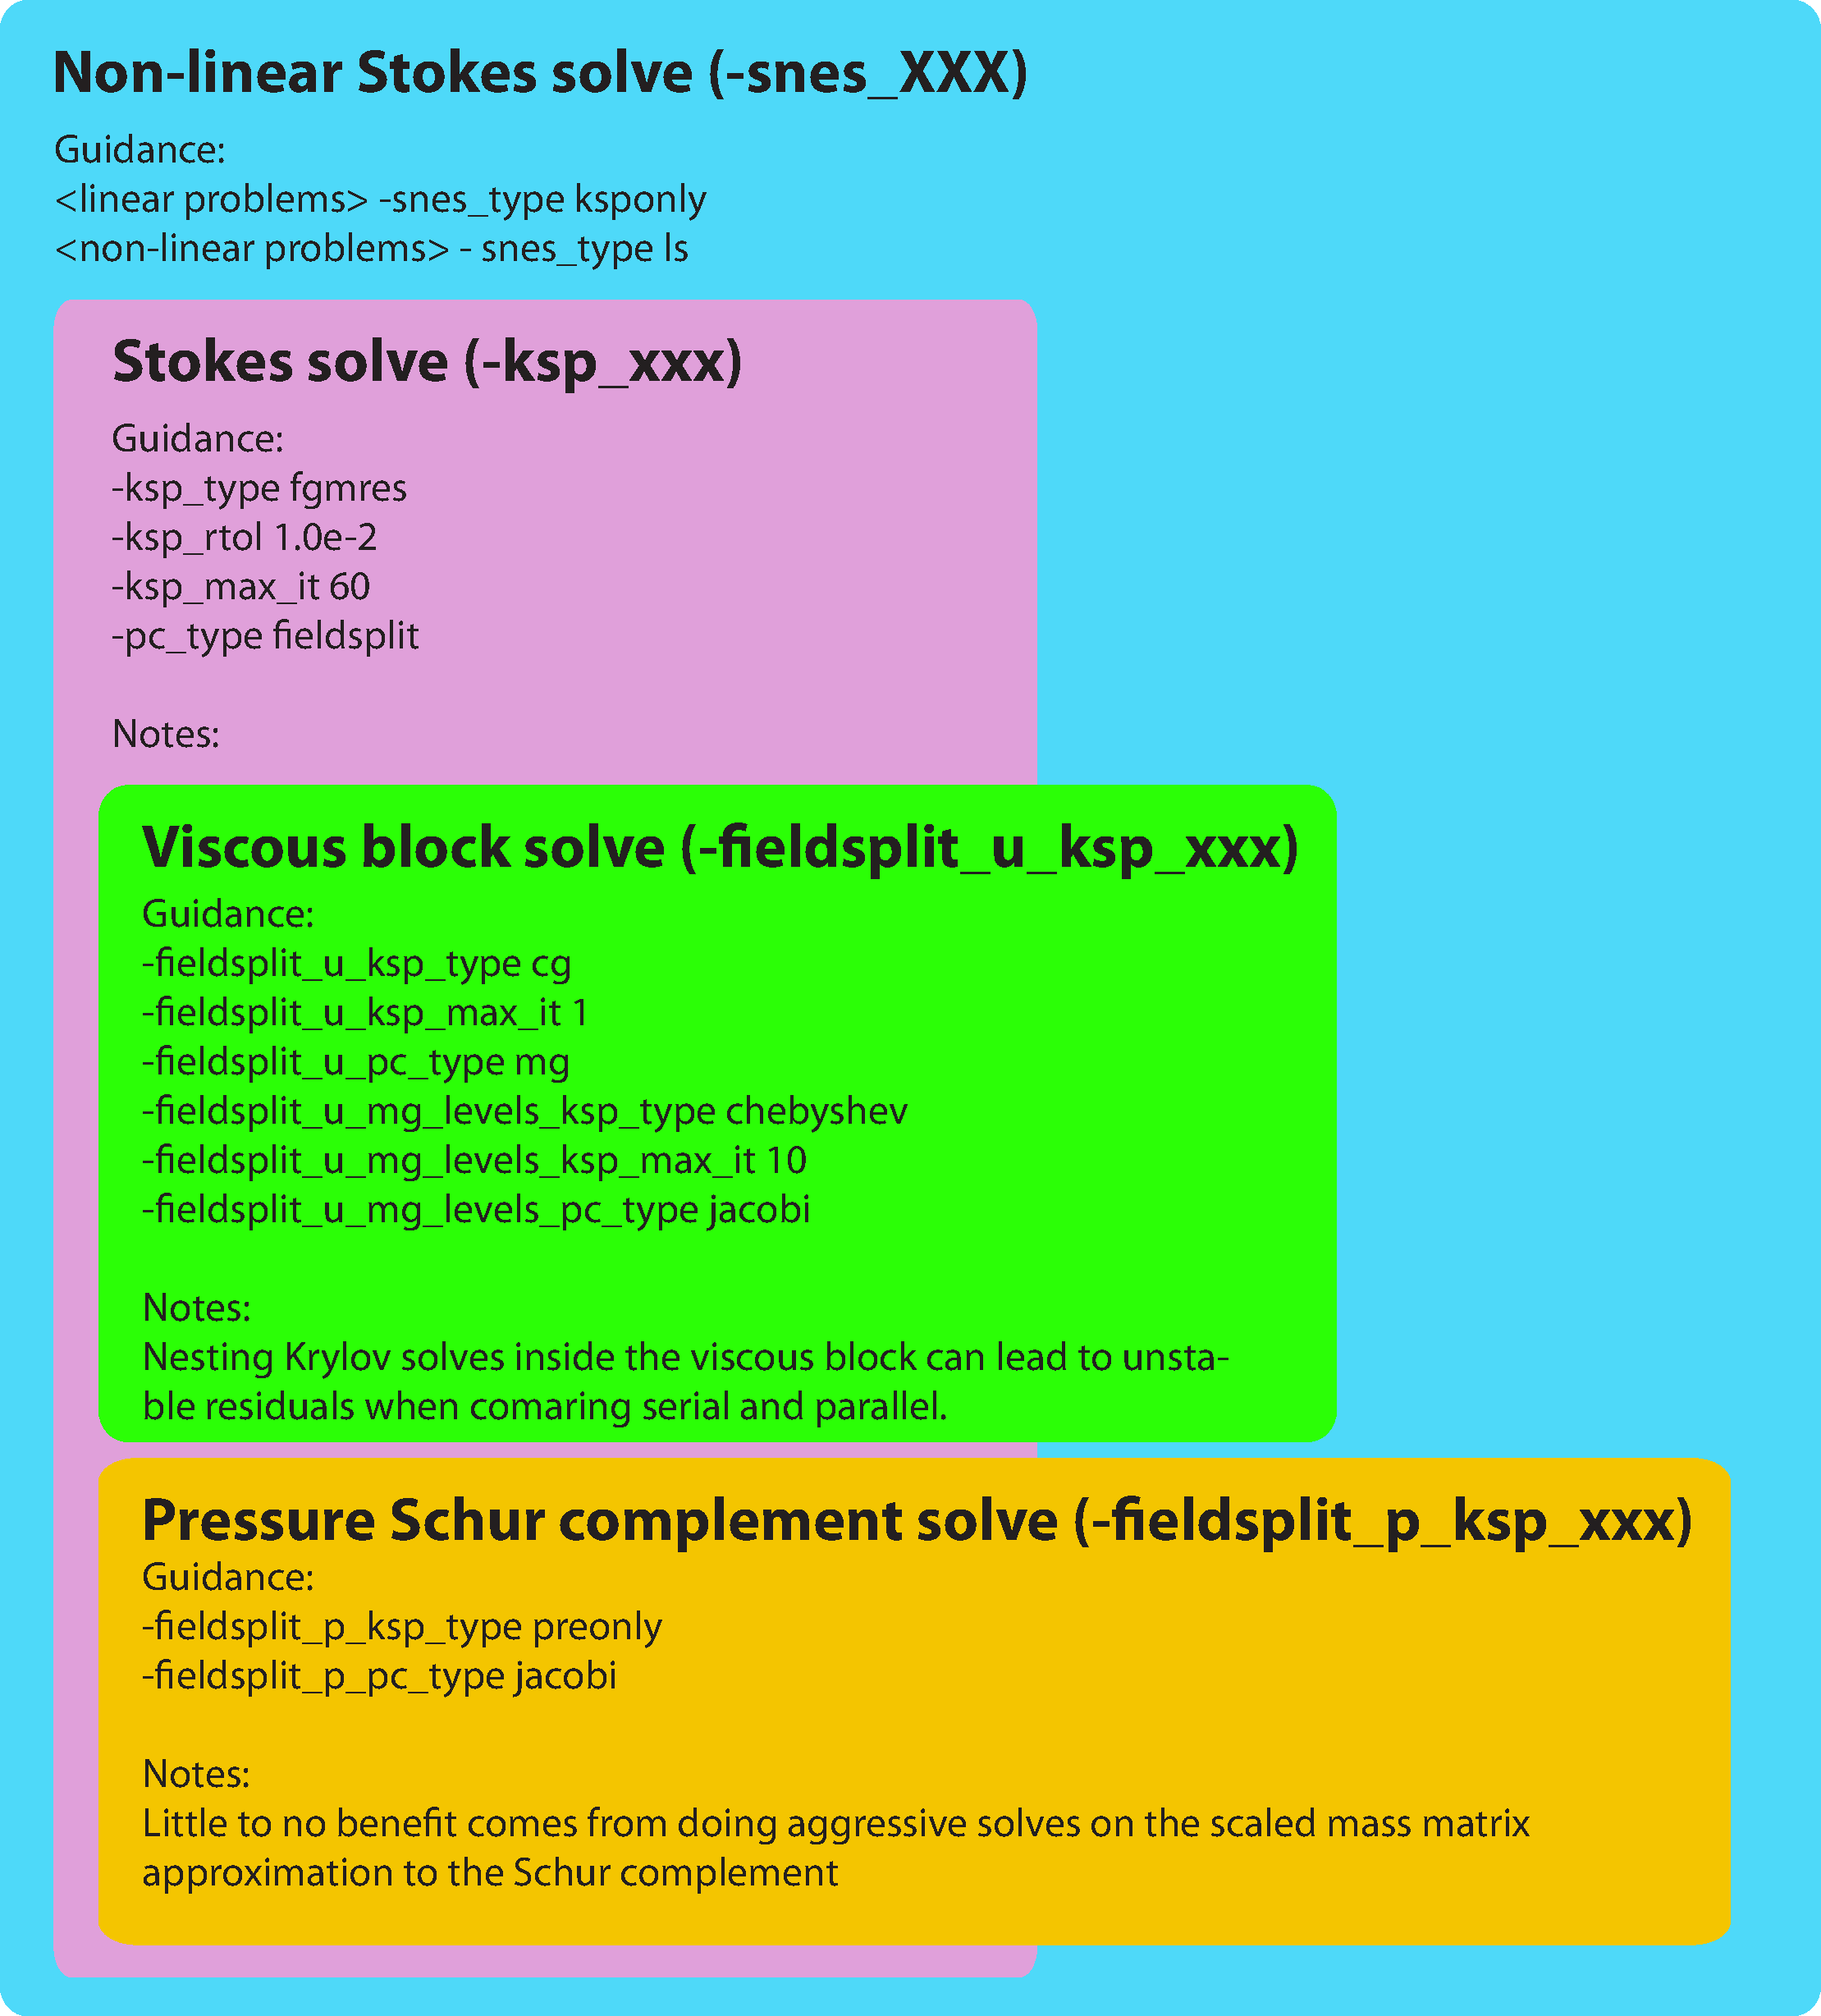
\includegraphics[height=0.6\textheight]{figs/pt3d_solve_hierarchy.pdf}
\caption[\itshape ]
{\itshape Solver hierarchy}
\label{fig:solver_hierarchy}
\end{figure}
In the following section we detail how to configure the solver applied to Eq.~\eqref{eq:discretelinearstokes_pc} to obtain $(u,p)$, and how to configure the solvers in steps 1 ({\tt -fieldsplit\_u\_ksp}) and 2 ({\tt -fieldsplit\_p\_ksp}) of applying the upper triangular preconditioner.


\subsection{Configuring solvers}



\subsection{Multi-grid sequencing}
The number of multi-grid levels is set via the option:
\shellcmd{-dau\_nlevels X}
If $X = 3$, this will imply that the mesh specified via \unix{-mx 16 -my 16 -mz 16} will be coarsened twice, resulting (by default) in a mesh sequence with the number of elements $M_x = 16$ (fine), $M_x = 8$ and $M_x = 4$ (coarse). For clarity, level 0 is designated as the ``coarsest'' level, and level $X-1$ is designated as the ``finest'' level.

Meshes can be coarsened by a constant factor on each level, or one can control the coarsening factor level-by level.
In both cases, the coarsening applied is dependent on the coordinate direction $(i,j,k)$. 
To define constant coarsening on every level, but varying in each direction, use the options
\shellcmd{-da\_refine\_x 4\\
\indent\indent\texttt{\hspace{5mm}}-da\_refine\_y 2 \\
\indent\indent\texttt{\hspace{5mm}}-da\_refine\_z 1}
Note that different coarsening can be specified in each direction - here denoted via $x,y,z$ in the refinement command line option.
Also note, that a refinement factor of 1 implies that mesh will not be coarsened in that direction. 

To define level specific coarsening, use the options
\shellcmd{-stk\_velocity\_da\_refine\_hierarchy\_x 4,1}
The integer parameters are listed from coarse to fine levels (left to right). The above options will result result in the following hierarchy in the $x$ direction (from coarse to fine), $M_x = \{ 4, 16, 16 \}$.
Note that if you have $X$ levels, you are only required to specify $X-1$ values to define the coarsening hierarchy. 


Note that when using geometric multi-grid, all levels are spatial decomposed across all cores. Furthermore, it is required that every core contains at least one element. Thus, the total number of cores used to run a {\ptat} job must not exceed the number of elements within the coarse grid. If you require additional levels in your multi-grid hierarchy, we recommend you use an algebraic multi-grid preconditioner as your coarse grid preconditioner.

\subsection{Coarse grid operators}
Within {\ptat}, the style of coarse grid operator can be configured at run time. We provide support to enable three types of coarse grid operator; $\{$ matrix-free re-discretised = 0, assembled re-discretised = 1, Galerkin = 2 $\}$. Re-discretised operators imply that the viscosity is projected through the mesh hierarchy and the finite element operators are re-evaluated using the standard FE weak form defined on the fine level. Galerkin coarsening implies that the coarse grid operator at level $k$ $A_k$ is defined via $A_k = R^T A_{k+1} R$, where $R$ is the restriction operator for level $k+1$ to $k$. To define the triple matrix product required by the a Galerkin operator definition on level $k$, it is require that the operator on level $k+1$ be assembled, i.e. be of either type $\{$ assembled re-discretised = 1, Galerkin = 2 $\}$. Configuration of the coarse grid operator type is define via the option;
\shellcmd{-A11\_operator\_type 2,2,1,0}
where valid indices are $\{ 0, 1, 2 \}$ and operators on each level are specified from coarse to fine (left to right).



\subsection{Multi-grid performance profiling}
To activate monitors which report CPU times on each mult-grid level, one must specify the following options
\shellcmd{-dau\_nlevels X -fieldsplit\_u\_pc\_type mg -fieldsplit\_u\_pc\_mg\_levels X -fieldsplit\_u\_pc\_mg\_log -log\_summary}
Note that if the values for \unix{-dau\_nlevels X} and \unix{-fieldsplit\_u\_pc\_mg\_levels X} do not match, logging will not be performed.


\subsection{Understanding residuals}

When solving linear problems, two types of residuals are important to monitor for both accuracy of the Stokes problem and efficiency of the solver.
By default, all drivers report the Stokes residuals for the individual components of the residual associated with the $u,v,w$-momentum equations and the continuity equation. The complete residual associated with the residual of the full vector $(u,v,w,p)$ can be monitored using the flag
\shellcmd{-ksp\_monitor}

The residuals output to the screen will typically look like the following:
\begingroup
    \fontsize{6.5pt}{6.5pt}\selectfont
	\begin{verbatim}
  0 KSP Component U,V,W,P residual norm [ 0.000000000000e+00, 2.307691625955e-03, 0.000000000000e+00, 0.000000000000e+00 ]
        Residual norms for fieldsplit_u_ solve.
        0 KSP Residual norm 1.000000000000e+00 
        1 KSP Residual norm 9.566218971472e-01 
        2 KSP Residual norm 6.120179419948e-01 
        3 KSP Residual norm 2.693954462485e-01 
        4 KSP Residual norm 7.305148723409e-02 
        5 KSP Residual norm 2.484961341074e-02 
        6 KSP Residual norm 7.872576358279e-03 
  1 KSP Component U,V,W,P residual norm [ 1.931850895378e-07, 2.249650371310e-03, 1.931669353791e-07, 3.613480131486e-04 ]
        Residual norms for fieldsplit_u_ solve.
        0 KSP Residual norm 9.383540923375e-01 
        1 KSP Residual norm 2.353199854638e-01 
        2 KSP Residual norm 6.233285019473e-02 
        3 KSP Residual norm 2.466199083002e-02 
        4 KSP Residual norm 6.082964600394e-03 
  2 KSP Component U,V,W,P residual norm [ 2.862389390637e-05, 9.461315464033e-04, 2.873233657833e-05, 1.128984116051e-03 ]
        Residual norms for fieldsplit_u_ solve.
        0 KSP Residual norm 1.461862868221e+01 
        1 KSP Residual norm 6.787824394358e-01 
        2 KSP Residual norm 1.306125161069e-01 
  3 KSP Component U,V,W,P residual norm [ 1.614279704240e-04, 4.795734857592e-04, 1.613914106944e-04, 8.488885268501e-04 ]
        Residual norms for fieldsplit_u_ solve.
        0 KSP Residual norm 3.614067424860e+01 
        1 KSP Residual norm 1.727513541857e+00 
        2 KSP Residual norm 1.701193913599e-01 
  4 KSP Component U,V,W,P residual norm [ 1.182053444264e-04, 2.177408865879e-04, 1.181950335293e-04, 3.963394470286e-04 ]
	\end{verbatim}
\endgroup
The longer lines containing the ``{\tt U,V,W,P residual norm}'' relate to the residuals of the Stokes problem, whilst the shorter lines under each instance of ``{\tt Residual norms for fieldsplit\_u\_ solve.}'' relate to the viscous block solver which is performed as the Stokes preconditioner is applied.


\section{Geometry}

\subsection{Modelling domain}
The underlying coordinate system used in {\ptat} is Cartesian. In Fig.~\ref{fig:domain_coord} we identify the face labels used.
\begin{figure} [hbtp]
\center
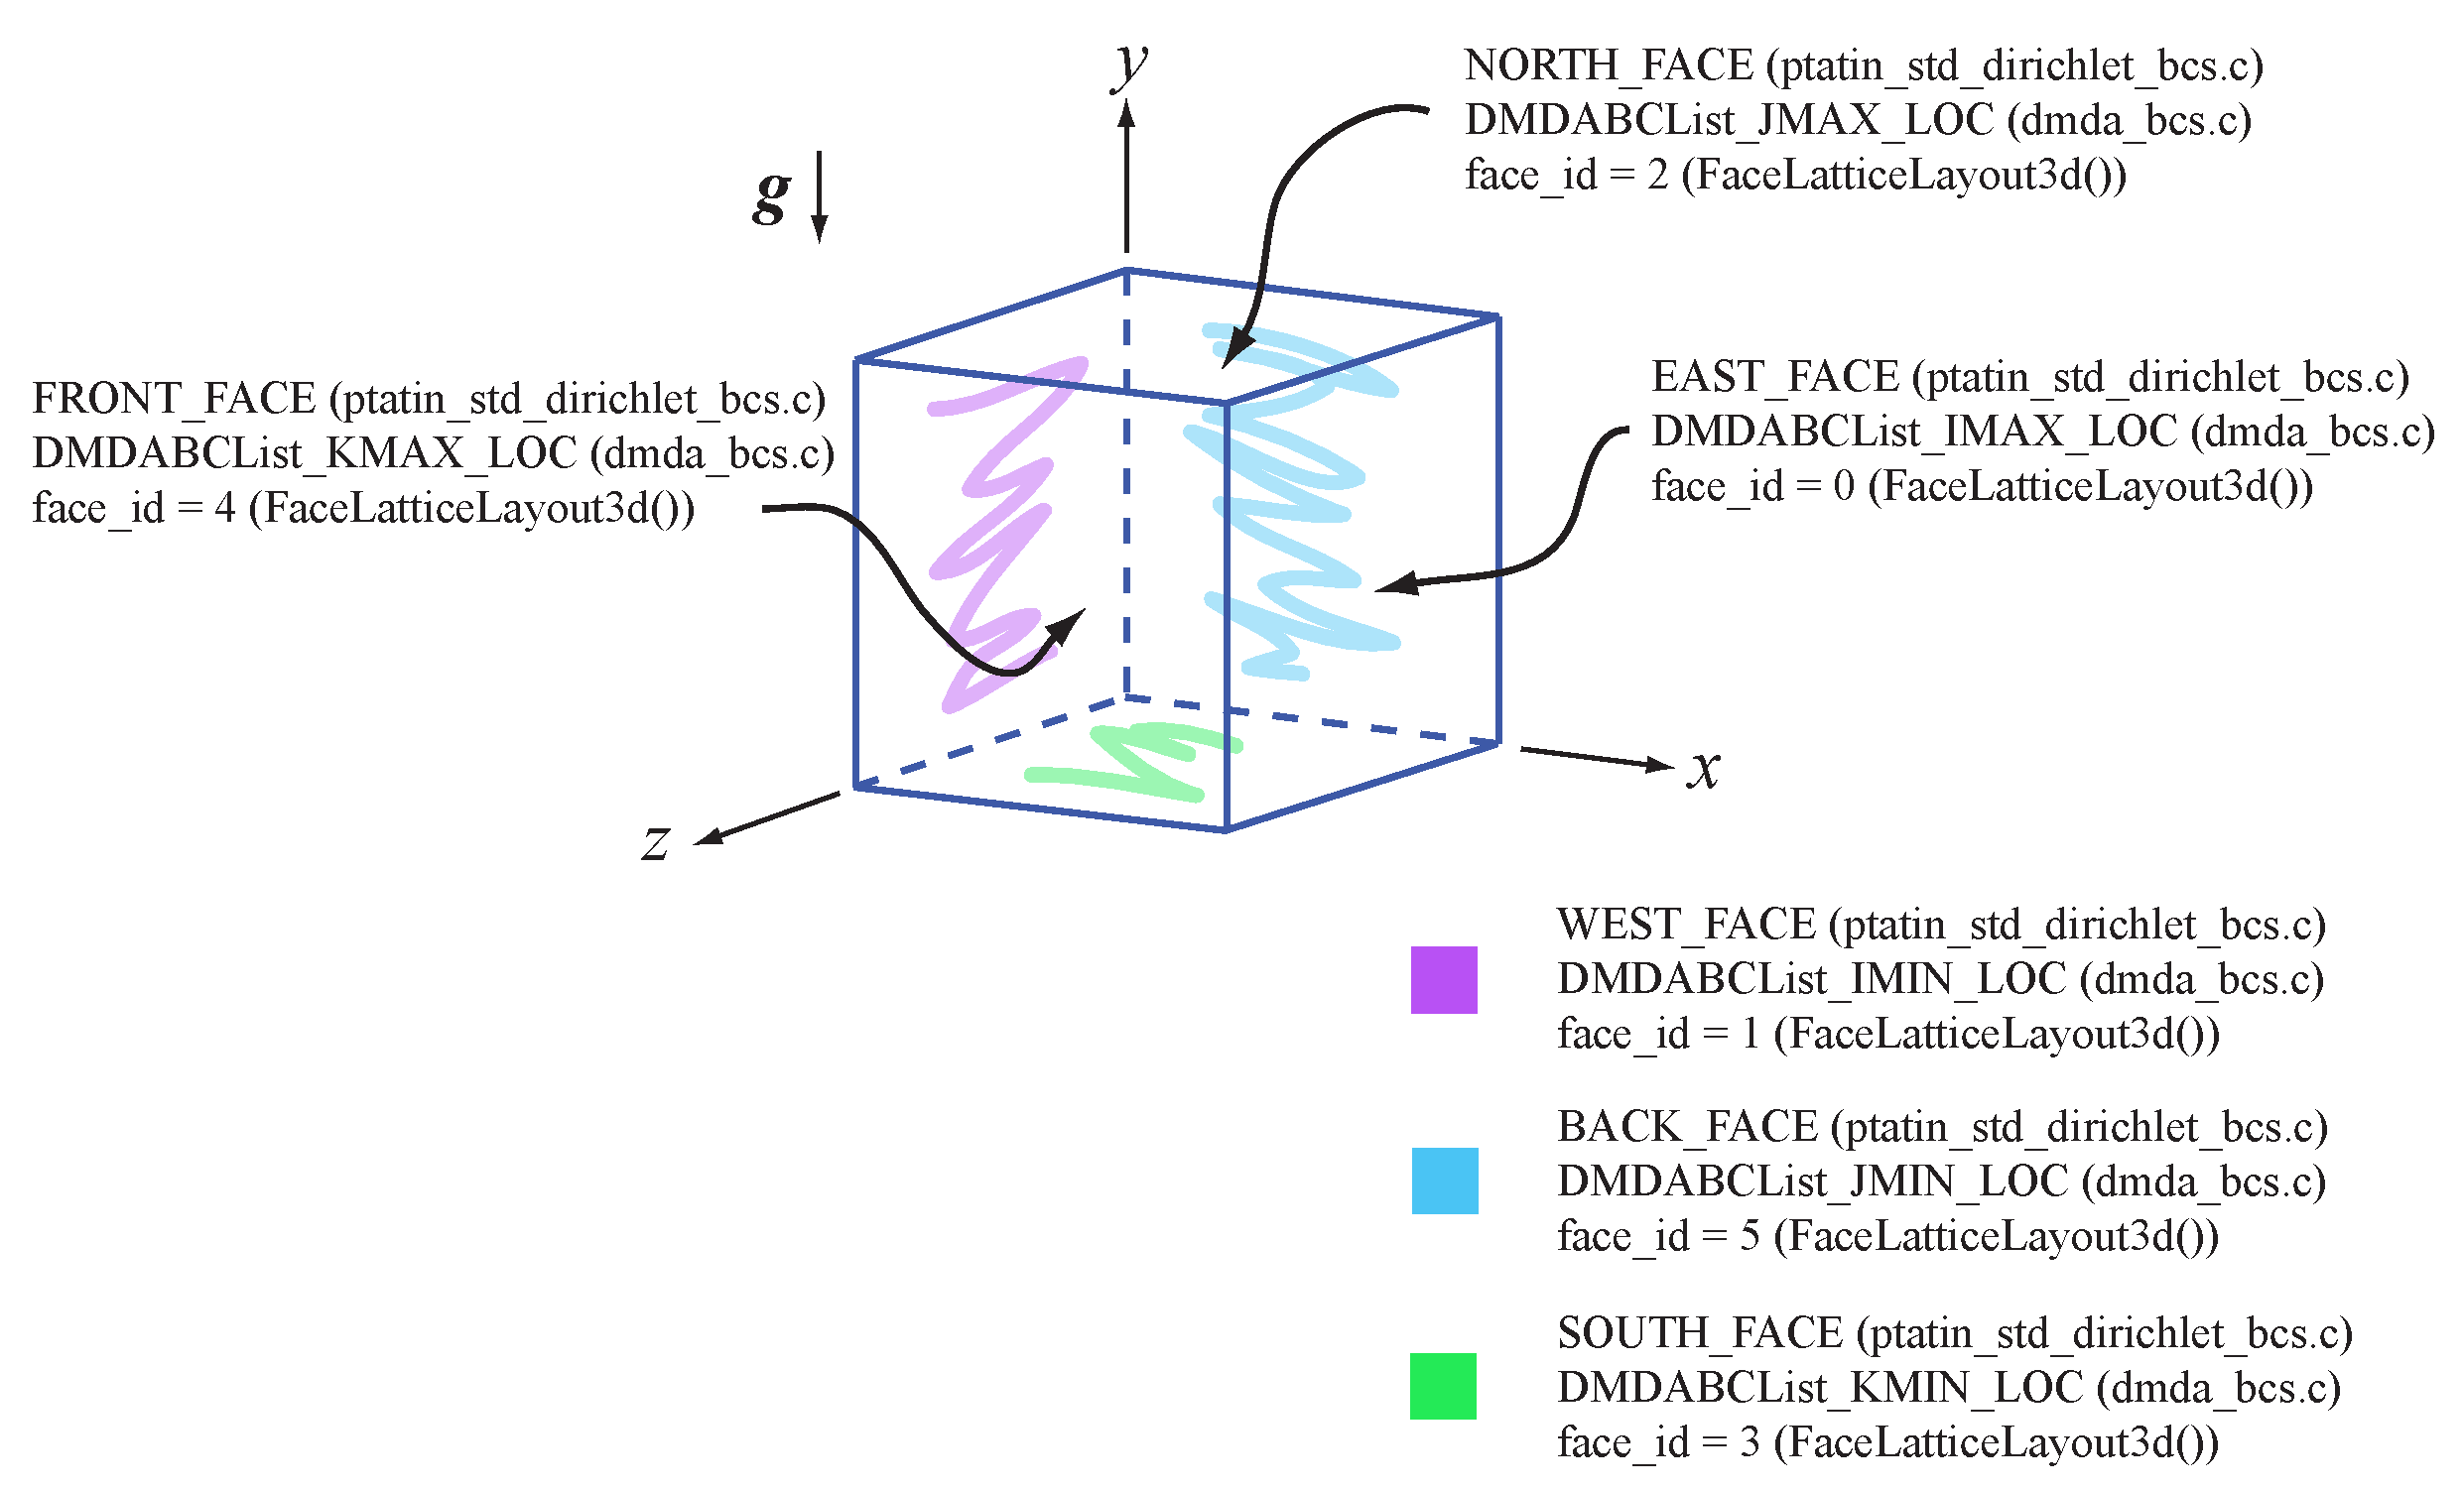
\includegraphics[height=0.4\textheight]{figs/pt3d_coordinate_system.pdf}
\caption[\itshape ]
{\itshape Natural coordinate system used by the physical domain $\Omega$ in {\ptat}. Labels indicate various names given by different structures functionality.}
\label{fig:domain_coord}
\end{figure}

\begin{figure} [hbtp]
\center
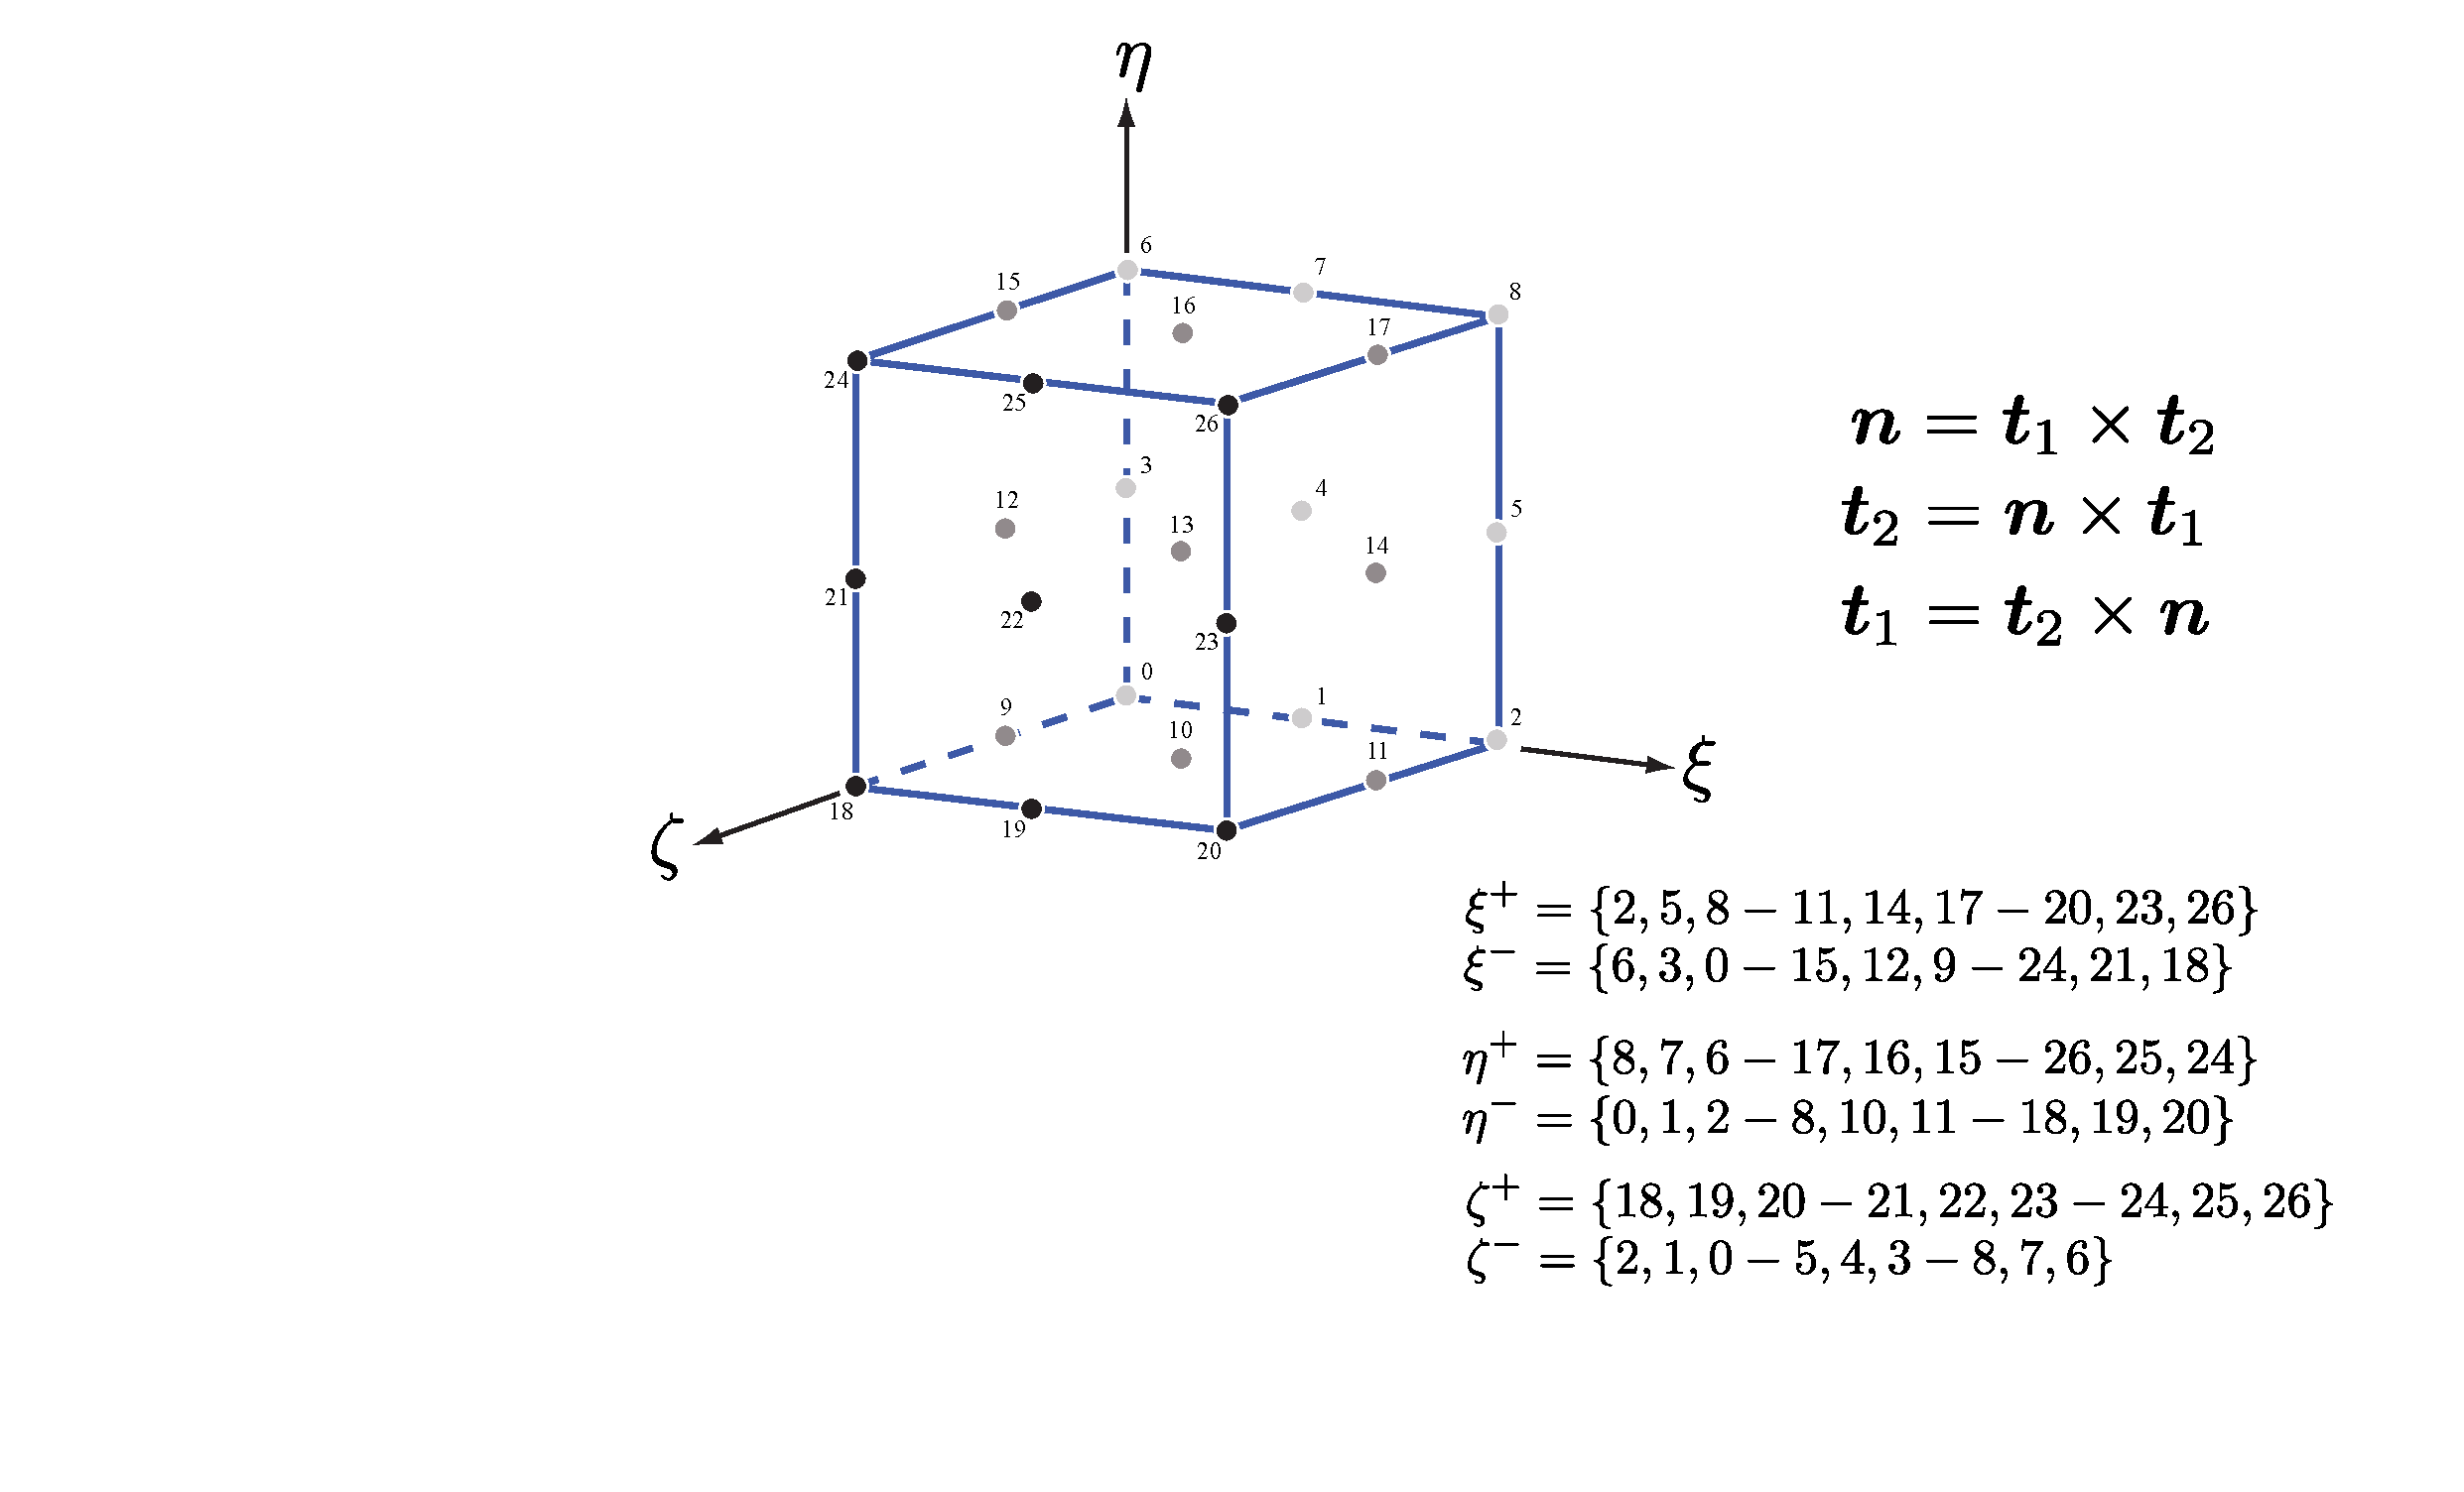
\includegraphics[height=0.4\textheight]{figs/pt3d_basis_functions.pdf}
\caption[\itshape ]
{\itshape Nomenclature and basis function ordering for the volume and surface basis functions. $\xi, \eta, \zeta$ are the spatial coordinates in local element coordinate system. The notation $\xi^{+}, \xi^{-}$ indicates faces along which $\xi = 1, \xi = -1$ respectively. The convention associated with defining outward pointing surface normals $(\boldsymbol n)$ and the two tangent vectors to the surface $(\boldsymbol t_1,\boldsymbol t_2)$ are indicated.}
\label{fig:basis_functions}
\end{figure}

\subsection{Defining geometric regions on material points}


\end{document}